% PairPulse manuscript formatted from the author's CAS double-column template.
\documentclass[a4paper,fleqn]{cas-dc}

\usepackage[numbers]{natbib}
\usepackage{amsmath,amssymb,bm}
\usepackage{graphicx}
\usepackage{booktabs}
\usepackage{xurl}
\usepackage{hyperref}
\hypersetup{hidelinks,
  pdftitle={A Reproducible Computational Framework for Fermion Pair Production in Pulsed Electric Fields},
  pdfauthor={Othman H. Y. Zalloum}}
\usepackage{xcolor}
\usepackage[switch]{lineno}
\setlength{\emergencystretch}{1em}
\usepackage{float}
\usepackage{placeins}
\usepackage{caption}
\captionsetup[figure]{skip=4pt}
\graphicspath{{../results/}}
\ExplSyntaxOn
\RenewDocumentCommand \printorcid { } { }
\ExplSyntaxOff

\def\tsc#1{\csdef{#1}{\textsc{\lowercase{#1}}\xspace}}
\tsc{WGM}
\tsc{QE}

\newcommand{\sech}{\operatorname{sech}}
\newcommand{\PairPulse}{\textsc{PairPulse}}

\begin{document}
\let\WriteBookmarks\relax
\def\floatpagepagefraction{1}
\def\textpagefraction{.001}

\shorttitle{Fermion Pair Production in Pulsed Electric Fields}
\shortauthors{Zalloum}
\title [mode = title]{A Reproducible Computational Framework for Fermion Pair Production in Pulsed Electric Fields}

\author[1]{Othman H. Y. Zalloum}
\cormark[1]
\ead{ozalloum@ppu.edu}
\ead[url]{https://orcid.org/0000-0001-7282-1332}
\affiliation[1]{organization={Palestine Polytechnic University},
            addressline={Department of Applied Mathematics and Physics},
            city={Hebron},
            country={Palestine}}
\cortext[1]{Corresponding author}

\begin{abstract}
We present \PairPulse, a reproducible computational program for momentum-resolved fermion pair production in prescribed, spatially homogeneous electric fields in one spatial dimension. For each canonical momentum, it independently evolves a two-component Dirac mode and the equivalent non-Markovian quantum-kinetic system. The exact asymptotic occupation for a temporal Sauter pulse supplies an external benchmark, while the Dirac norm and quantum-kinetic Bloch-vector invariant provide independent integration diagnostics. The program supports superpositions of temporally displaced Sauter pulses and user-defined pulse objects through a compact field--potential interface. For $E_0/m^2=0.3$ and $m\tau=2$, both solvers reproduce the analytic occupation on 41 momentum points with maximum absolute error below $8\times10^{-13}$. A supplementary suite of 2,228 mode evaluations separates integration, endpoint and momentum-grid errors. Nine Sauter parameter pairs give maximum absolute occupation error $4.58\times10^{-15}$ at refined settings, and comparison with QuTiP 5.2.2 gives differences below $8.27\times10^{-16}$ for the single- and double-pulse spectra. Momentum-grid and domain refinements meet a declared $10^{-4}$ relative density criterion. A momentum--window map shows the absolute finite-window discrepancy across the benchmark grid. A separated two-pulse calculation demonstrates the workflow for a field for which the package supplies no closed-form spectrum. The contribution is a transparent reference implementation with tests, data, and figure-generation scripts; no new pair-production mechanism or analytic result is claimed.
\end{abstract}

\begin{highlights}
\item Evolves Dirac modes and quantum-kinetic equations independently.
\item Benchmarks both solvers against the exact temporal-Sauter spectrum.
\item Reports norm, invariant, pulse-tail, and cross-formulation diagnostics.
\item Maps absolute finite-window error over momentum and tail extent.
\item Includes tested code, reproducible data, figures, and a notebook.
\end{highlights}

\begin{keywords}
Schwinger mechanism \sep quantum kinetic theory \sep Dirac equation \sep time-dependent electric fields \sep pair production \sep reproducible scientific software
\end{keywords}

\maketitle
\linenumbers

\section*{Program summary}
\noindent\textbf{Program title:} \PairPulse\\
\textbf{CPC library link to program files:} Not yet assigned.\\
\textbf{Developer's repository link:} \url{https://github.com/ozalloum/PairPulse}.\\
\textbf{Code Ocean capsule:} Not applicable.\\
\textbf{Licensing provisions:} MIT License.\\
\textbf{Programming language:} Python 3.10 or later.\\
\textbf{External routines/libraries:} NumPy and SciPy; Matplotlib for plots.\\
\textbf{Nature of problem:} Momentum-resolved fermion pair occupation in a prescribed, spatially homogeneous, time-dependent electric field in 1+1 dimensions.\\
\textbf{Solution method:} Adaptive DOP853 integration of two equivalent but independently implemented state systems: the two-component Dirac equation and the non-Markovian quantum-kinetic equations. The exact temporal-Sauter solution, Dirac norm, quantum-kinetic invariant, and cross-formulation agreement are used for validation.\\
\textbf{Restrictions:} One fermion species in one spatial dimension. Spatial gradients, transverse momentum, collisions, back-reaction, photon dynamics, and self-consistent Maxwell evolution are not included.\\
\textbf{Unusual features:} The exact benchmark and two state representations are combined with independent conservation checks. Scripts regenerate the manuscript figures, tables, and run metadata.

\section{Introduction}

Nonperturbative pair creation by electric fields is a foundational prediction of quantum electrodynamics. Its early development includes the effective-action treatment of vacuum polarization, Dirac-state transmission in a uniform field, and pair creation in constant or alternating backgrounds \cite{EulerHeisenberg1936,Sauter1931,Schwinger1951,BrezinItzykson1970}. Time-dependent mean-field and kinetic descriptions subsequently clarified how pair occupations evolve, how Pauli blocking enters, and when memory effects matter \cite{Kluger1991,Kluger1992,Kluger1998,Schmidt1998,Schmidt1999}.

For pulsed fields, the final momentum spectrum depends on the full time history of the background. Non-Markovian quantum-kinetic calculations have been compared with scattering and effective-action approaches, and the temporal Sauter field provides an especially useful exact reference case \cite{Hebenstreit2008,Schutzhold2008,Dumlu2009,Hebenstreit2010,Fedotov2011,Huet2014}. Short pulses and subcycle structure produce characteristic momentum signatures, while semiclassical turning-point analyses explain interference patterns in time-dependent backgrounds \cite{Hebenstreit2009,DumluDunne2010,DumluDunne2011a,DumluDunne2011b,Akkermans2012,Li2014}. These studies make clear why a numerical implementation should specify its in/out convention, integration window, and momentum variable rather than report a spectrum without those choices.

Several complementary computational approaches address broader field configurations and observables. Reviews summarize the strong-field and quantum-kinetic setting; real-time lattice simulations treat dynamical fermion production; and later work examines pulse-shape effects, spatially varying fields, and the validity of the spatially uniform approximation \cite{DiPiazza2012,Hebenstreit2013,GelisTanji2016,Aleksandrov2016,Aleksandrov2017a,Aleksandrov2017b,Lv2018,Aleksandrov2018}. The definition of particle number during a field pulse also depends on the chosen basis, a point clarified by analyses of adiabatic particle number \cite{Ilderton2022}. This motivates a narrowly specified benchmark calculation rather than an unqualified claim of general applicability.

This paper introduces \PairPulse, a compact computational-physics program that evolves two independently represented mode systems under the same prescribed field: a two-component Dirac spinor and the non-Markovian quantum-kinetic variables. The exact asymptotic Sauter spectrum provides an external benchmark; conservation diagnostics test each integration internally; and a two-pulse example checks cross-formulation agreement beyond the exactly soluble case. The package includes the source, automated tests, a reproduction notebook, generated figures, machine-readable data, and run metadata. It is intended as a transparent reference implementation for method checks and modest parameter studies in the spatially homogeneous model, and it does not claim new pair-production physics.


Existing software provides useful comparisons. The RODARE release of Edwards et al.\ \cite{EdwardsSoftware2025} supplies MATLAB code and datasets for hierarchy-expanded relativistic quantum-kinetic calculations in time-dependent fields. Its documented aim is to resolve contributions in assisted pair production. QuTiP is a general quantum-dynamics framework with time-dependent Hamiltonian solvers \cite{Lambert2026}. PairPulse packages a narrower workflow: paired Dirac and full auxiliary-variable kinetic evolution, a common in/out convention, an exact Sauter benchmark, conservation diagnostics, and reproducible spectra and density checks. This integration is its practical contribution; no claim of software priority or superiority over the wider capabilities of these packages is made. The RODARE comparison concerns documented scope, whereas QuTiP 5.2.2 is executed as a separate numerical comparator below.

The remainder of the paper defines the field and mode conventions, describes the software and numerical method, reports validation results, and states the scope and limitations of the program.

\section{Physical model}
\label{sec:model}

We use natural units, $\hbar=c=1$, and temporal gauge, $A^0=0$. The positive charge magnitude is denoted by $q$; reversing the charge is equivalent to reflecting canonical momentum for the backgrounds considered here. For a spatially uniform vector potential $A(t)$, the kinetic momentum of a mode with canonical momentum $p$ is
\begin{equation}
  \pi_p(t)=p-qA(t), \qquad E(t)=-\dot A(t).
  \label{eq:kinetic}
\end{equation}
The default pulse is
\begin{align}
  E(t)&=E_0\sech^2\!\left(\frac{t-t_c}{\tau}\right),\nonumber\\
  A(t)&=-E_0\tau\tanh\!\left(\frac{t-t_c}{\tau}\right).
  \label{eq:sauter}
\end{align}
with $E_0\geq0$. A pulse train is formed by summing the fields and the corresponding potentials. This preserves Eq.~\eqref{eq:kinetic} without numerical integration of the electric field.

\subsection{Dirac-mode evolution}

After reduction to a two-component mode, the Hamiltonian can be written
\begin{equation}
  H_p(t)=\pi_p(t)\sigma_1+m\sigma_3, \qquad
  i\partial_t\psi_p(t)=H_p(t)\psi_p(t),
  \label{eq:dirac}
\end{equation}
where $m>0$ and $\sigma_i$ are Pauli matrices. At the initial and final times, where the pulse tails are small, the instantaneous negative- and positive-energy eigenvectors define the in-vacuum and the out-particle state. The occupation is
\begin{equation}
  f_p=\left|u_{p,+}^{\dagger}(t_f)\psi_p(t_f)\right|^2,
  \label{eq:occupation}
\end{equation}
with $\psi_p(t_i)=u_{p,-}(t_i)$. Exact evolution preserves $\psi_p^\dagger\psi_p=1$.

\subsection{Quantum-kinetic evolution}

The second formulation evolves the distribution $f_p$ and two auxiliary functions $u_p,v_p$. Defining $\omega_p(t)=\sqrt{m^2+\pi_p(t)^2}$ and $W_p(t)=qE(t)m/\omega_p(t)^2$, the equations are
\begin{align}
  \dot f_p &= \frac{1}{2}W_p u_p, \nonumber\\
  \dot u_p &= W_p(1-2f_p)-2\omega_p v_p, \label{eq:qke}\\
  \dot v_p &= 2\omega_p u_p, \nonumber
\end{align}
with $(f_p,u_p,v_p)=(0,0,0)$ at the finite initial time $t_i$. This represents the instantaneous vacuum used by the Dirac solver, and approaches the asymptotic in-vacuum as the pulse tails vanish. The local auxiliary-variable system represents the non-Markovian kinetic evolution \cite{Schmidt1998,Dumlu2009}. These equations preserve
\begin{equation}
  (1-2f_p)^2+u_p^2+v_p^2=1,
  \label{eq:invariant}
\end{equation}
which is used as an independent integration diagnostic. The asymptotic value of $f_p$ is compared directly with Eq.~\eqref{eq:occupation}.

\subsection{Exact Sauter benchmark}

For Eq.~\eqref{eq:sauter}, let $\lambda=qE_0\tau^2$ and
\begin{equation}
  \omega_{\pm}=\sqrt{m^2+(p\pm qE_0\tau)^2}.
\end{equation}
The asymptotic occupation per fermionic mode, with no additional spin-degeneracy factor, is \cite{Hebenstreit2010}
\begin{equation}
  f_p^{\mathrm{exact}}=
  \frac{\cosh(2\pi\lambda)-
  \cosh\!\left[\pi\tau(\omega_+-\omega_-)\right]}
  {2\sinh(\pi\tau\omega_+)\sinh(\pi\tau\omega_-)}.
  \label{eq:exact}
\end{equation}
The spin-summed distribution in Ref.~\cite{Hebenstreit2010}, Eq.~(99), is twice the per-mode occupation used here, with transverse momentum set to zero. This normalization is consistent with the single-species density below. The implementation evaluates an algebraically equivalent logarithmic expression to reduce overflow in the hyperbolic functions. This algebraic reformulation does not guarantee relative accuracy for arbitrarily small occupations. Equation~\eqref{eq:exact} is used only for a single Sauter pulse; pulse-train spectra are computed by time evolution.

\section{Software and numerical method}
\label{sec:software}

\PairPulse{} is a Python package built around a small pulse interface exposing $E(t)$, $A(t)$, and a finite integration window. It provides an analytic Sauter pulse and finite pulse trains, but the solvers accept user-defined pulse objects implementing the same interface. This separates the field model from the mode evolution and lets users replace the pulse without changing either solver.

Both initial-value problems use SciPy's DOP853 solver through \texttt{solve\_ivp}. The default relative and absolute tolerances are $2\times10^{-10}$ and $2\times10^{-12}$. The integration window extends 12 duration parameters beyond the outermost pulse centers by default. For each mode, 257 equally spaced times in $[t_i,t_f]$ are used to estimate $\omega_{\max}=\max\sqrt{m^2+[p-qA(t)]^2}$, and the maximum internal step is $c_h/\omega_{\max}$, where the public parameter \texttt{max\_step\_coefficient} defaults to $c_h=0.18$. This sampled cap is empirical; it is not a rigorous frequency bound for an arbitrary user-defined pulse. The window length is user-adjustable; the manuscript's tail study makes its effect explicit. The same time interval, DOP853 implementation, tolerances, and step-cap rule are used for both formulations. Thus the state equations are implemented independently, but their time integrator is shared. Agreement between them does not by itself exclude common integration or window errors. Custom pulse objects must supply mutually consistent $E(t)$ and $A(t)$ with sufficiently decayed endpoint fields; the interface does not check these conditions automatically.

For a single Sauter pulse, \PairPulse{} reports the exact occupation, direct Dirac occupation, quantum-kinetic occupation, final-time norm/invariant errors, and ODE function-evaluation counts. These diagnostics are not maxima over the intermediate time history. The two reproduction scripts regenerate the six manuscript figures, comma-separated tables, and environment metadata. The additional \texttt{redraw\_figures.py} script redraws the figures directly from the archived CSVs without new mode integrations. The accompanying notebook shows the central benchmark and pulse-train example. The eight tests cover the exact benchmark, the quantum-kinetic invariant and occupation bounds, the zero-field limit, pulse superposition, time translation, step-cap refinement, and rejection of invalid controls or nonfinite pulse parameters.

Figures~\ref{fig:package} and \ref{fig:workflow} summarize the public package contents and the sequence used to regenerate its datasets and publication figures. Both diagrams are generated by the included Python plotting script. The separate finite-window scan writes its underlying momentum--tail-extent values to a CSV file, in addition to the spectra, convergence data, and run metadata produced by the main reproduction script.

The one-dimensional momentum-integrated density is defined as
\begin{equation}
  n_{1\mathrm{D}}=\int\frac{dp}{2\pi}f_p,
  \label{eq:density}
\end{equation}
and is evaluated with the trapezoidal rule on the supplied finite momentum grid. It is a one-dimensional density for one mode species, not a three-dimensional number density. Users must check momentum-window and grid convergence for applications beyond the examples below.

\FloatBarrier
\section{Results}
\label{sec:results}

\subsection{Single Sauter pulse}

The reference case uses $m=q=1$, $E_0=0.3$, $\tau=2$, and 41 equally spaced canonical momenta on $[-1.5,1.5]$. Figure~\ref{fig:sauter} compares both numerical formulations with Eq.~\eqref{eq:exact}. Across this grid, the largest absolute errors are $7.48\times10^{-13}$ for the Dirac modes and $7.54\times10^{-13}$ for the quantum-kinetic calculation. The maximum relative errors over modes with $f_p^{\mathrm{exact}}>10^{-12}$ are $1.68\times10^{-8}$ and $1.68\times10^{-8}$, respectively. The maximum final-time Dirac norm error across the momentum grid is $6.24\times10^{-13}$; the maximum final-time deviation of the quantum-kinetic invariant from unity is $9.13\times10^{-13}$.

\begin{figure}[pos=htbp]
  \centering
  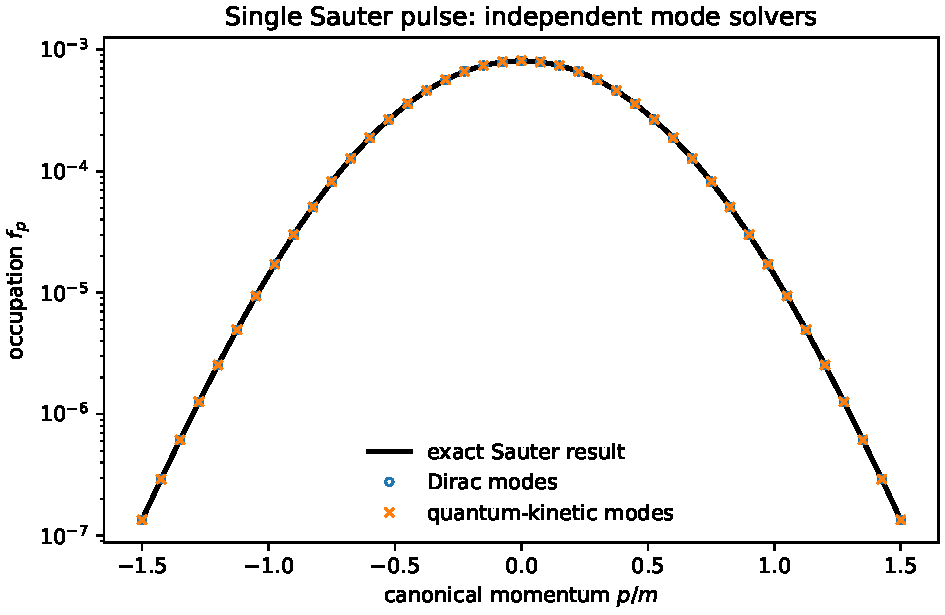
\includegraphics[width=0.78\linewidth]{figure1_sauter_validation.pdf}
  \caption{Single-pulse occupation spectrum for $E_0=0.3$, $\tau=2$, $t_c=0$, and $m=q=1$, evaluated at 41 equally spaced canonical momenta in $[-1.5,1.5]$. The black line is the exact asymptotic Sauter result; circles and crosses denote Dirac and quantum-kinetic modes integrated over $[-12\tau,12\tau]$. The numerical results lie on the exact curve at this resolution. The vertical axis is logarithmic; markers represent deterministic calculations, with no statistical error bars.}
  \label{fig:sauter}
\end{figure}

At the fixed solver settings used here, short integration windows give larger discrepancies from the asymptotic benchmark. At $p=0$ the exact value is $8.11991615993\times10^{-4}$. Table~\ref{tab:tail} shows that extending the window from six to twelve pulse durations reduces the absolute error by more than five orders of magnitude. At $14\tau$, discrepancies are of order $10^{-14}$. This scan alone cannot separate residual tail error from integration error and roundoff; Section~\ref{sec:refinement} reports separate refinements.

\begin{table*}[pos=tp]
  \centering
  \small
  \caption{Finite-window convergence at $p=0$ for $E_0=0.3$, $\tau=2$, $t_c=0$, and $m=q=1$. Endpoints are $t_i=-L$, $t_f=L$. Both solvers use relative tolerance $2\times10^{-10}$, absolute tolerance $2\times10^{-12}$, and the step cap in Section~\ref{sec:software}. Errors are absolute differences from Eq.~\eqref{eq:exact}; numerical tolerances are held fixed as $L$ varies.}
  \label{tab:tail}
  \begin{tabular}{rrrr}
    \toprule
    Tail half-width $L/\tau$ & Exact & Dirac absolute error & QKE absolute error\\
    \midrule
    6  & $8.11991615993\times10^{-4}$ & $1.1762\times10^{-7}$ & $1.1762\times10^{-7}$\\
    8  & $8.11991615993\times10^{-4}$ & $2.1989\times10^{-9}$ & $2.1989\times10^{-9}$\\
    10 & $8.11991615993\times10^{-4}$ & $4.0728\times10^{-11}$ & $4.0721\times10^{-11}$\\
    12 & $8.11991615993\times10^{-4}$ & $7.4813\times10^{-13}$ & $7.5435\times10^{-13}$\\
    14 & $8.11991615993\times10^{-4}$ & $1.2825\times10^{-14}$ & $6.7149\times10^{-15}$\\
    \bottomrule
  \end{tabular}
\end{table*}

\subsection{Separated pulses}

As a case for which the package supplies no closed-form benchmark, we superpose two same-polarity Sauter pulses, each with $E_0=0.3$ and $\tau=1.1$, centered at $t_c=\pm3.5$. Figure~\ref{fig:double} shows the computed momentum spectrum on $[-1.8,1.8]$. The two independent state representations agree over the full grid; both resolve shoulders and modulations away from the central maximum. The spectrum is included as a cross-formulation code demonstration. Its detailed features are not assigned to a specific interference mechanism on the basis of this calculation alone.

\begin{figure}[pos=htbp]
  \centering
  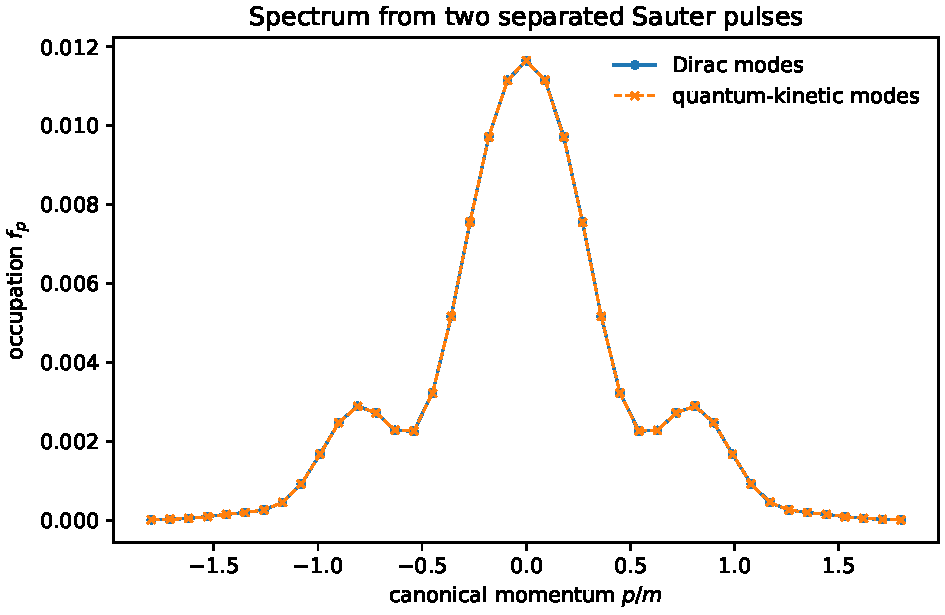
\includegraphics[width=0.78\linewidth]{figure2_double_pulse.pdf}
  \caption{Occupation spectrum for two separated, same-polarity Sauter pulses, each with $E_0=0.3$ and $\tau=1.1$, centered at $t_c=\pm3.5$, with $m=q=1$. Circles with a solid line and crosses with a dashed line denote Dirac and quantum-kinetic calculations on 41 equally spaced canonical momenta in $[-1.8,1.8]$. Endpoints are $t_i=-16.7$, $t_f=16.7$. Lines join computed modes; no analytic curve is supplied for this case.}
  \label{fig:double}
\end{figure}

The largest absolute difference between the Dirac and quantum-kinetic occupations on this grid is $1.18\times10^{-13}$. For orientation, trapezoidal integration over the stated finite windows gives $n_{1\mathrm{D}}=1.13951\times10^{-4}$ for the single-pulse exact spectrum and $1.69199\times10^{-3}$ for the double-pulse spectrum. These original values use the finite grids shown in the figures. Section~\ref{sec:densityvalidation} separately refines the momentum spacing and domain.

\subsection{Evolution diagnostics}

Figure~\ref{fig:invariant} displays the absolute quantum-kinetic invariant error for the single-pulse momentum grid. The maximum error is below $10^{-12}$ in this run. The invariant is a useful internal diagnostic, but it does not replace comparison with the exact occupation or a convergence study in momentum and time.

\begin{figure}[pos=htbp]
  \centering
  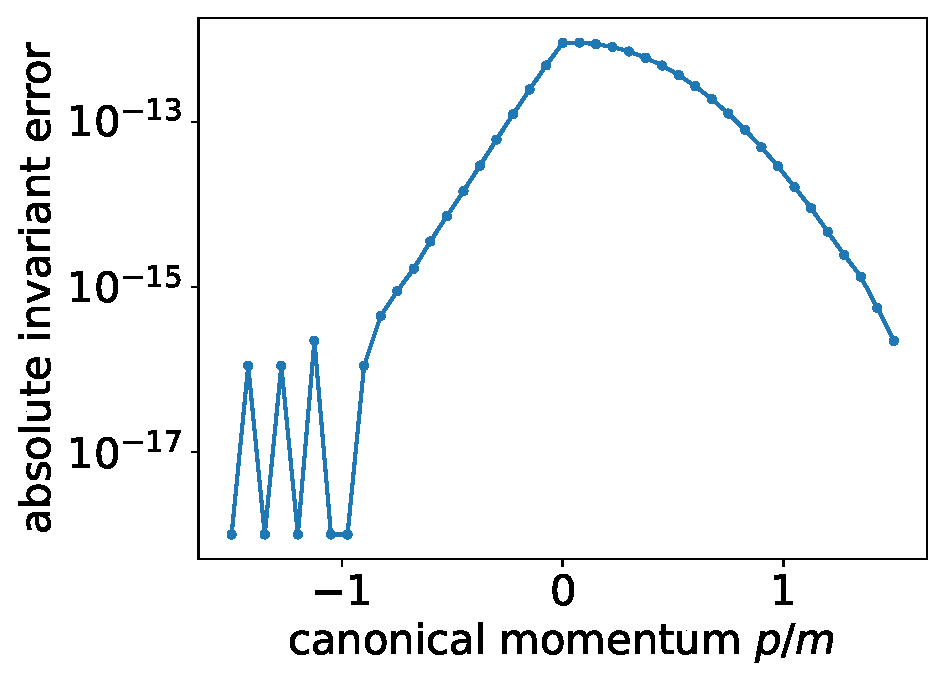
\includegraphics[width=0.78\linewidth]{figure3_qke_invariant.pdf}
  \caption{Final-time quantum-kinetic invariant error $|(1-2f_p)^2+u_p^2+v_p^2-1|$ for the single-pulse setup of Figure~\ref{fig:sauter}. Each marker corresponds to one of 41 momentum modes, evaluated at $t_f=12\tau$; the connecting line guides the eye. Values are plotted on a logarithmic scale with a display floor of $10^{-18}$. The diagnostic measures conservation of the invariant, not occupation error or a maximum over time.}
  \label{fig:invariant}
\end{figure}

Short integration windows can shift the computed spectrum away from its asymptotic value. Figure~\ref{fig:window-error} shows the absolute error for both formulations. The scan uses 41 momenta and six tail half-widths, with $L/\tau$ from 4 to 14 in steps of 2. Parameters are $E_0/m^2=0.3$ and $m\tau=2$.

Here $L$ is the half-width from the pulse center to either integration endpoint. The plotted discrepancy includes finite-window truncation and fixed-tolerance integration error; small discrepancies are not necessarily pure tail error. The CSV records both occupations, the exact result, errors, and solver diagnostics. Because the field is spatially homogeneous, the map axes are momentum and window extent.

\begin{figure*}[pos=tp]
  \centering
  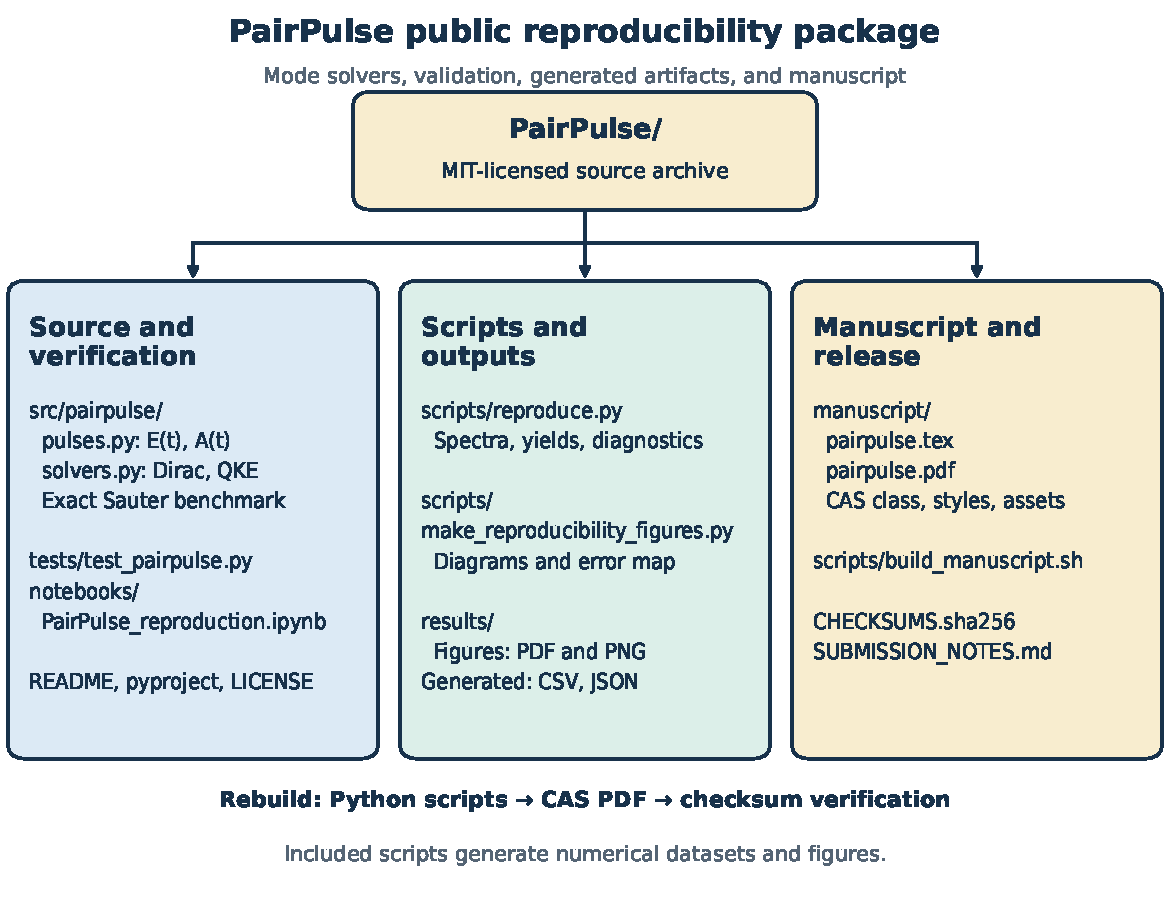
\includegraphics[width=\textwidth]{figure4_reproducibility_structure.pdf}
  \caption{Structure of the public \PairPulse{} package. Source modules, tests, notebook, and run scripts are shown alongside the generated datasets, figures, manuscript, and release checks. The diagram is produced in Python from the package's declared file structure.}
  \label{fig:package}
\end{figure*}

\begin{figure*}[pos=tp]
  \centering
  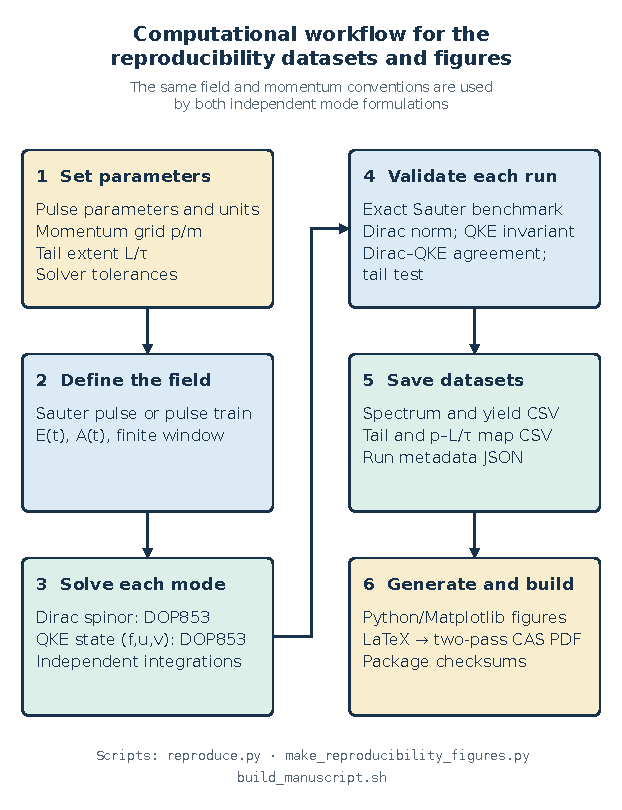
\includegraphics[width=\textwidth]{figure5_computational_workflow.pdf}
  \caption{Computational workflow used to generate the reproducibility datasets and publication figures. Each momentum mode is evolved independently with the Dirac and quantum-kinetic systems; the exact Sauter result and conservation diagnostics are then used where applicable before data export, plotting, and manuscript compilation.}
  \label{fig:workflow}
\end{figure*}

\begin{figure*}[pos=tp]
  \centering
  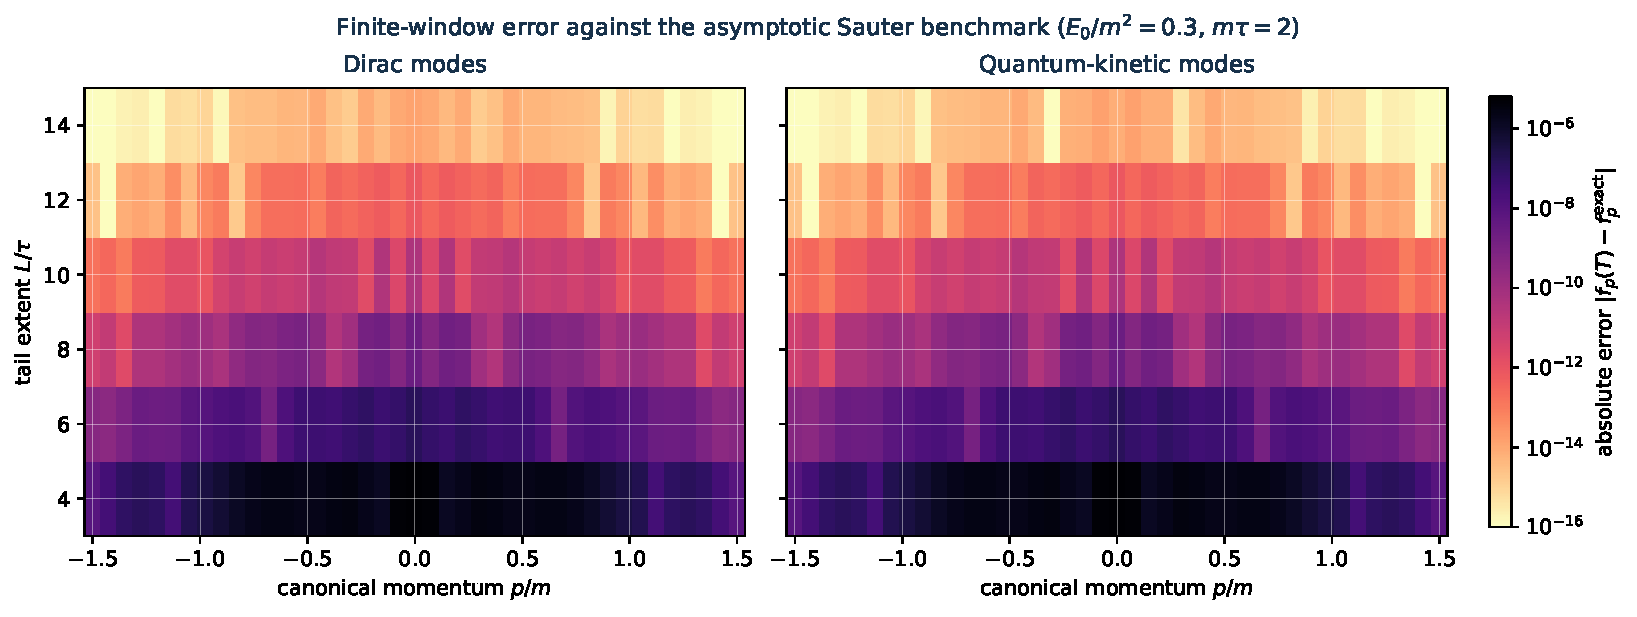
\includegraphics[width=0.94\textwidth]{figure6_sauter_window_error_map.pdf}
  \caption{Absolute finite-window discrepancy $|f_p(L)-f_p^{\mathrm{exact}}|$ from the asymptotic Sauter benchmark: (a) Dirac modes and (b) quantum-kinetic modes, for $E_0=0.3$, $\tau=2$, $t_c=0$, and $m=q=1$. Each panel contains 41 momenta in $[-1.5,1.5]$ and six half-widths $L/\tau=4,6,8,10,12,14$; integration endpoints are $t_c\pm L$. The common logarithmic color scale uses a display floor of $10^{-16}$ without changing the archived errors. Discrepancies include window, integration, and roundoff effects at fixed tolerances. The horizontal coordinate is canonical momentum, not position.}
  \label{fig:window-error}
\end{figure*}


\subsection{Validation protocol and integration refinement}
\label{sec:refinement}

A supplementary validation suite contains 2,228 individual mode evaluations, all completed without integration failures. The protocol was recorded before execution. Its acceptance criteria are occupation differences below $10^{-10}$, relative errors below $10^{-5}$ when the exact occupation is at least $10^{-10}$, successive relative changes below $10^{-4}$ for the integrated density, and no occupation outside $[0,1]$ by more than $10^{-10}$. These are empirical acceptance criteria, not certified error bounds. Every mode, solver setting, diagnostic and failure field is retained in \path{validation/mode_results.csv}; the scripts retain unsuccessful integrations rather than silently discarding them.

At fixed tail extent 20, each of the single- and double-pulse cases is tested at $p=0$, $p=\pm0.75$ and $p=\pm1.5$. The relative tolerance takes values $2\times10^{-8}$, $2\times10^{-10}$ and $2\times10^{-12}$, with absolute tolerance one hundredth as large; independently, $c_h$ takes values 0.18, 0.09 and 0.045. Both formulations are run at all combinations (180 evaluations). The largest occupation difference from the same formulation at the tightest tolerance and cap is $8.46\times10^{-14}$. Refinement differences need not decrease monotonically once errors approach floating-point precision. The refined double-pulse solution is a numerical reference, not an exact solution.

Separately, 60 evaluations vary the tail extent through 12, 16 and 20 at relative tolerance $2\times10^{-12}$ and $c_h=0.045$. Relative to extent 20, the largest occupation differences at extent 12 are $7.48\times10^{-13}$ for the single pulse and $2.59\times10^{-13}$ for the double pulse; at extent 16 they are below $2.51\times10^{-16}$ and $9.37\times10^{-16}$, respectively. This distinguishes endpoint sensitivity from the fixed-window integration study.

\subsection{Parameter coverage and a custom pulse}

The Sauter benchmark is evaluated at all nine combinations of $E_0=0.1,0.3,0.8$ and $\tau=0.5,2,5$, with $m=q=1$. Each uses 13 equally spaced momenta on $[-p_{\max},p_{\max}]$, where $p_{\max}=\max(1.5,E_0\tau+2/\tau)$, tail extent 20, relative tolerance $2\times10^{-12}$, absolute tolerance $2\times10^{-14}$ and $c_h=0.09$. Table~\ref{tab:parameter} reports all 234 evaluations. The largest absolute error is $4.58\times10^{-15}$, and the largest relative error over resolved occupations is $1.83\times10^{-9}$. No negative occupations or upper-bound violations occur in this sweep. Exact occupations reach $7.81\times10^{-19}$; relative accuracy is not asserted for these smallest values.

\begin{table}[pos=htbp]
\centering\small
\caption{Maximum absolute Sauter occupation error over 13 momenta per parameter pair, for each formulation. Settings are specified in the text.}
\label{tab:parameter}
\begin{tabular}{rrrr}\toprule
$E_0$ & $\tau$ & Dirac & QKE\\\midrule
0.1 & 0.5 & $4.84\times10^{-17}$ & $8.19\times10^{-16}$\\
0.1 & 2 & $4.02\times10^{-18}$ & $1.71\times10^{-18}$\\
0.1 & 5 & $8.39\times10^{-20}$ & $4.12\times10^{-19}$\\
0.3 & 0.5 & $9.71\times10^{-17}$ & $2.71\times10^{-15}$\\
0.3 & 2 & $5.43\times10^{-17}$ & $2.76\times10^{-17}$\\
0.3 & 5 & $5.90\times10^{-17}$ & $9.67\times10^{-18}$\\
0.8 & 0.5 & $4.27\times10^{-15}$ & $4.58\times10^{-15}$\\
0.8 & 2 & $6.45\times10^{-16}$ & $1.77\times10^{-16}$\\
0.8 & 5 & $1.54\times10^{-15}$ & $1.42\times10^{-16}$\\
\bottomrule\end{tabular}
\end{table}

A user-defined Gaussian profile provides an additional interface check:
\begin{align}
E(t)&=0.3\exp[-(t/2)^2],\nonumber\\
A(t)&=-0.3\sqrt{\pi}\,\operatorname{erf}(t/2).
\end{align}
These expressions satisfy $E=-\dot A$. Five momenta, two endpoint extents ($|t|=12,16$), two cap coefficients (0.09, 0.045) and three solvers give 60 evaluations. Differences from the longest-window, smallest-cap QuTiP result are below $3.53\times10^{-17}$. This checks one smooth custom profile and does not validate arbitrary user-supplied fields.

\subsection{Comparison with QuTiP}

QuTiP 5.2.2 \cite{Lambert2026} evolves the two-level Hamiltonian in Eq.~\eqref{eq:dirac} using \texttt{sesolve} with the \texttt{vern9} integrator. Its endpoint eigensystems and state evolution are constructed independently of PairPulse's right-hand side and eigenvector helper. The analytic potential, physical conventions and endpoint times are shared. Automatic output normalization is disabled so that norm drift remains observable. The run uses tail extent 20, relative tolerance $2\times10^{-12}$, absolute tolerance $2\times10^{-14}$ and $c_h=0.09$ on the same 41 momenta as each original spectrum, giving 246 evaluations across the three solvers.

\begin{table}[pos=htbp]
\centering\small
\caption{Largest absolute occupation difference from QuTiP on 41 modes per case. These compare refined runs, not the original default-setting curves.}
\label{tab:software}
\begin{tabular}{lrr}\toprule
Case & Dirac--QuTiP & QKE--QuTiP\\\midrule
Single pulse & $1.09\times10^{-16}$ & $9.06\times10^{-17}$\\
Double pulse & $8.27\times10^{-16}$ & $4.11\times10^{-16}$\\
\bottomrule\end{tabular}
\end{table}

For the single pulse, QuTiP's maximum absolute error against the analytic result is $1.04\times10^{-16}$. Table~\ref{tab:software} supplies an executed comparison using a different integration implementation. The shared field specification remains a common assumption. No matched-accuracy runtime comparison is claimed: wall times retained from concurrent validation workers are execution records, not controlled performance benchmarks.

\subsection{Momentum-grid and domain refinement}
\label{sec:densityvalidation}

The QKE density is first evaluated at 41, 81 and 161 nodes on the original fixed momentum interval. The spacing of the 161-node grid is then held constant as the interval is doubled and tripled, using 321 and 481 nodes. All modes are evaluated directly, without imposing spectrum symmetry. A nested 481-node grid per case supplies the 962 mode evaluations in this study. Tail extent 20, relative tolerance $2\times10^{-12}$, absolute tolerance $2\times10^{-14}$ and $c_h=0.09$ are used throughout.

\begin{table}[pos=htbp]
\centering\small
\caption{Trapezoidal density refinement. $P$ is the half-width of the momentum interval and $N_p$ is its number of nodes. All values use QKE.}
\label{tab:density}
\begin{tabular}{lrrr}\toprule
Case & $P$ & $N_p$ & $n_{1\mathrm D}$\\\midrule
Single & 1.5 & 41 & $1.1395114844\times10^{-4}$\\
 & 1.5 & 81 & $1.1395130337\times10^{-4}$\\
 & 1.5 & 161 & $1.1395134244\times10^{-4}$\\
 & 3.0 & 321 & $1.1395539392\times10^{-4}$\\
 & 4.5 & 481 & $1.1395539392\times10^{-4}$\\
Double & 1.8 & 41 & $1.6919881473\times10^{-3}$\\
 & 1.8 & 81 & $1.6919976391\times10^{-3}$\\
 & 1.8 & 161 & $1.6920000711\times10^{-3}$\\
 & 3.6 & 321 & $1.6926588379\times10^{-3}$\\
 & 5.4 & 481 & $1.6926588400\times10^{-3}$\\
\bottomrule\end{tabular}
\end{table}

The last fixed-domain grid refinement changes the single- and double-pulse densities by $3.43\times10^{-7}$ and $1.44\times10^{-6}$ relatively. The final domain extension changes them by $7.20\times10^{-13}$ and $1.21\times10^{-9}$, respectively. The largest difference between the QKE and analytic single-pulse densities on identical grids is below $1.71\times10^{-18}$. A further 486 mode evaluations on 81-node grids vary tail extents (12, 16, 20) and halve the cap coefficient at extent 20; the largest relative density change is $4.98\times10^{-11}$. The density checks therefore meet the declared $10^{-4}$ criterion, while remaining finite refinement evidence rather than a rigorous continuum error estimate.

\subsection{Installation and execution records}

The numerical suite was executed on 8 October 2026 with Python 3.12.14, NumPy 2.3.5, SciPy 1.17.0 and QuTiP 5.2.2. Machine and dependency metadata accompany the data. A built wheel was installed into two isolated Windows environments: Python 3.12.14 with the reproduction libraries, and Python 3.10.20 with NumPy 1.24.0, SciPy 1.10.0 and Matplotlib 3.7.0. All eight tests passed in both environments. Separate hosted checks successfully built and installed the package from source on Linux and Windows. On both systems, the notebook executed all four code cells in a real Jupyter kernel, imported the installed package, and produced no error outputs. Execution records identify the tested revisions, dependencies and notebook hashes; the earlier restricted local Windows kernel failure is retained separately.

\FloatBarrier
\section{Limitations and intended use}

The implementation assumes a prescribed, spatially homogeneous background and one spatial dimension. It does not include back-reaction, collisions, spatial gradients, transverse momentum, scalar particles, or a self-consistent electromagnetic field. This restriction is physically consequential: calculations beyond the dipole or spatially uniform approximation show that field variation can change pair yields and momentum spectra \cite{Aleksandrov2016,Aleksandrov2017b,Lv2018,Aleksandrov2018}. \PairPulse{} is therefore a reference implementation for the stated homogeneous model, not a substitute for lattice, Wigner, or spatially resolved calculations when these effects matter.

The exact Sauter formula validates asymptotic occupation for a single pulse; it does not validate every user-supplied field. For new profiles, users should vary tolerances, pulse-tail windows, time-step limits, and momentum resolution, and compare physical observables with an independent method where possible. Particle-number interpretation during an active pulse requires particular care because instantaneous occupation can be basis dependent \cite{Ilderton2022}.

The supplementary studies separate integration controls, endpoint extent, momentum spacing and momentum range, and cover nine single-pulse parameter pairs plus a Gaussian profile. This finite set does not establish a parameter-independent accuracy bound. Very weak occupations, stronger or longer pulses, sharply structured custom fields and larger pulse trains require further checks.


The code emphasizes clarity and cross-validation over throughput. Each momentum mode is integrated independently in Python, so the present package is most appropriate for reference calculations, method checks, and modest parameter sweeps. The validation script can distribute independent modes among subprocess workers. Compiled kernels and demonstrated scaling for large parameter scans remain outside the current assessment.

\section{Conclusion}

\PairPulse{} provides an inspectable implementation of two established formulations for fermion pair creation in homogeneous pulsed electric fields. The exact Sauter solution, norm and invariant diagnostics, pulse-tail data, separated-pulse example, and executable notebook make the numerical conventions reproducible. The two numerical formulations reproduce the exact benchmark to below $8\times10^{-13}$ absolute error for the stated parameter set and agree to about $1.2\times10^{-13}$ for the two-pulse example. The additional 2,228 evaluations separate integration and domain errors, cover nine Sauter parameter pairs, test a custom Gaussian pulse, and compare against QuTiP with a different integrator. All declared numerical criteria pass. These results validate the implementation for the tested cases; they do not establish a general accuracy guarantee or claim new pair-production physics.

The deliberately limited model makes the package useful as a reference for homogeneous-field calculations and as a base for extensions. Applications involving spatial dependence, back-reaction, or additional particle degrees of freedom require further derivations and validation against appropriate independent methods.

\section*{Code and data availability}
The \PairPulse{} source code and numerical data supporting this study are available in the versioned snapshot v0.2.0 at \url{https://github.com/ozalloum/PairPulse/releases/tag/v0.2.0}. The release contains the Python solvers, unit tests, reproduction and figure-generation scripts, executable notebook, CSV data tables, generated figures, run metadata, and manuscript source and build files. Installation and reproduction instructions are provided in the repository README, and the data files and diagnostic conventions are described in \path{docs/DATA.md}. The PairPulse code is distributed under the MIT License; the bundled Elsevier CAS files retain their upstream license notices. A SHA-256 manifest identifies the distributed files. The release tag and associated commit identify this revision independently of subsequent changes to the main branch.

\section*{CRediT authorship contribution statement}
Othman H. Y. Zalloum: Conceptualization, Methodology, Software, Validation, Formal analysis, Investigation, Resources, Data curation, Visualization, Project administration, Writing--original draft, Writing--review and editing.

\section*{Funding}
This research did not receive any specific grant from funding agencies in the public, commercial, or not-for-profit sectors.

\section*{Acknowledgements}
The author acknowledges Palestine Polytechnic University for its support.

\section*{Declaration of competing interest}
The author declares that there are no known competing financial interests or personal relationships that could have appeared to influence the work reported in this paper.

\section*{Declaration of generative AI and AI-assisted technologies in the manuscript preparation process}
ChatGPT (OpenAI) was used to assist with manuscript editing, literature and reference checks, source-code inspection, plotting-script revisions, reproducibility checks, and LaTeX formatting. The scientific plots were generated with Python from numerical calculations or archived data. The corresponding author is responsible for reviewing and verifying the scientific content, computations, references, and final text before submission.

\begin{thebibliography}{99}
\bibitem{EulerHeisenberg1936}
W. Heisenberg and H. Euler, Folgerungen aus der Diracschen Theorie des Positrons, \textit{Zeitschrift f\"ur Physik} 98 (1936) 714--732. \url{https://doi.org/10.1007/BF01343663}.

\bibitem{Sauter1931}
F. Sauter, \"Uber das Verhalten eines Elektrons im homogenen elektrischen Feld nach der relativistischen Theorie Diracs, \textit{Zeitschrift f\"ur Physik} 69 (1931) 742--764. \url{https://doi.org/10.1007/BF01339461}.

\bibitem{Schwinger1951}
J. Schwinger, On gauge invariance and vacuum polarization, \textit{Physical Review} 82 (1951) 664--679. \url{https://doi.org/10.1103/PhysRev.82.664}.

\bibitem{BrezinItzykson1970}
E. Br\'ezin and C. Itzykson, Pair production in vacuum by an alternating field, \textit{Physical Review D} 2 (1970) 1191--1199. \url{https://doi.org/10.1103/PhysRevD.2.1191}.

\bibitem{Kluger1991}
Y. Kluger, J. M. Eisenberg, B. Svetitsky, F. Cooper, and E. Mottola, Pair production in a strong electric field, \textit{Physical Review Letters} 67 (1991) 2427--2430. \url{https://doi.org/10.1103/PhysRevLett.67.2427}.

\bibitem{Kluger1992}
Y. Kluger, J. M. Eisenberg, B. Svetitsky, F. Cooper, and E. Mottola, Fermion pair production in a strong electric field, \textit{Physical Review D} 45 (1992) 4659. \url{https://doi.org/10.1103/PhysRevD.45.4659}.

\bibitem{Kluger1998}
Y. Kluger, E. Mottola, and J. M. Eisenberg, Quantum Vlasov equation and its Markov limit, \textit{Physical Review D} 58 (1998) 125015. \url{https://doi.org/10.1103/PhysRevD.58.125015}.

\bibitem{Schmidt1998}
S. Schmidt, D. Blaschke, G. R\"opke, S. A. Smolyansky, A. V. Prozorkevich, and V. D. Toneev, A quantum kinetic equation for particle production in the Schwinger mechanism, \textit{International Journal of Modern Physics E} 7 (1998) 709--722. \url{https://doi.org/10.1142/S0218301398000403}.

\bibitem{Schmidt1999}
S. Schmidt, D. Blaschke, G. R\"opke, A. V. Prozorkevich, S. A. Smolyansky, and V. D. Toneev, Non-Markovian effects in strong-field pair creation, \textit{Physical Review D} 59 (1999) 094005. \url{https://doi.org/10.1103/PhysRevD.59.094005}.

\bibitem{Hebenstreit2008}
F. Hebenstreit, R. Alkofer, and H. Gies, Pair production beyond the Schwinger formula in time-dependent electric fields, \textit{Physical Review D} 78 (2008) 061701(R). \url{https://doi.org/10.1103/PhysRevD.78.061701}.

\bibitem{Schutzhold2008}
R. Sch\"utzhold, H. Gies, and G. Dunne, Dynamically assisted Schwinger mechanism, \textit{Physical Review Letters} 101 (2008) 130404. \url{https://doi.org/10.1103/PhysRevLett.101.130404}.

\bibitem{Dumlu2009}
C. K. Dumlu, Quantum kinetic approach and the scattering approach to vacuum pair production, \textit{Physical Review D} 79 (2009) 065027. \url{https://doi.org/10.1103/PhysRevD.79.065027}.

\bibitem{Hebenstreit2010}
F. Hebenstreit, R. Alkofer, and H. Gies, Schwinger pair production in space- and time-dependent electric fields: Relating the Wigner formalism to quantum kinetic theory, \textit{Physical Review D} 82 (2010) 105026. \url{https://doi.org/10.1103/PhysRevD.82.105026}.

\bibitem{Fedotov2011}
A. M. Fedotov, E. G. Gelfer, K. Yu. Korolev, and S. A. Smolyansky, Kinetic equation approach to pair production by a time-dependent electric field, \textit{Physical Review D} 83 (2011) 025011. \url{https://doi.org/10.1103/PhysRevD.83.025011}.

\bibitem{Huet2014}
A. Huet, S. P. Kim, and C. Schubert, Vlasov equation for Schwinger pair production in a time-dependent electric field, \textit{Physical Review D} 90 (2014) 125033. \url{https://doi.org/10.1103/PhysRevD.90.125033}.

\bibitem{Hebenstreit2009}
F. Hebenstreit, R. Alkofer, G. V. Dunne, and H. Gies, Momentum signatures for Schwinger pair production in short laser pulses with a subcycle structure, \textit{Physical Review Letters} 102 (2009) 150404. \url{https://doi.org/10.1103/PhysRevLett.102.150404}.

\bibitem{DumluDunne2010}
C. K. Dumlu and G. V. Dunne, Stokes phenomenon and Schwinger vacuum pair production in time-dependent laser pulses, \textit{Physical Review Letters} 104 (2010) 250402. \url{https://doi.org/10.1103/PhysRevLett.104.250402}.

\bibitem{DumluDunne2011a}
C. K. Dumlu and G. V. Dunne, Interference effects in Schwinger vacuum pair production for time-dependent laser pulses, \textit{Physical Review D} 83 (2011) 065028. \url{https://doi.org/10.1103/PhysRevD.83.065028}.

\bibitem{DumluDunne2011b}
C. K. Dumlu and G. V. Dunne, Complex worldline instantons and quantum interference in vacuum pair production, \textit{Physical Review D} 84 (2011) 125023. \url{https://doi.org/10.1103/PhysRevD.84.125023}.

\bibitem{Akkermans2012}
E. Akkermans and G. V. Dunne, Ramsey fringes and time-domain multiple-slit interference from vacuum, \textit{Physical Review Letters} 108 (2012) 030401. \url{https://doi.org/10.1103/PhysRevLett.108.030401}.

\bibitem{Li2014}
Z. L. Li, D. Lu, B. S. Xie, L. B. Fu, J. Liu, and B. F. Shen, Enhanced pair production in strong fields by multiple-slit interference effect with dynamically assisted Schwinger mechanism, \textit{Physical Review D} 89 (2014) 093011. \url{https://doi.org/10.1103/PhysRevD.89.093011}.

\bibitem{DiPiazza2012}
A. Di Piazza, C. M\"uller, K. Z. Hatsagortsyan, and C. H. Keitel, Extremely high-intensity laser interactions with fundamental quantum systems, \textit{Reviews of Modern Physics} 84 (2012) 1177. \url{https://doi.org/10.1103/RevModPhys.84.1177}.

\bibitem{Hebenstreit2013}
F. Hebenstreit, J. Berges, and D. Gelfand, Simulating fermion production in 1+1 dimensional QED, \textit{Physical Review D} 87 (2013) 105006. \url{https://doi.org/10.1103/PhysRevD.87.105006}.

\bibitem{GelisTanji2016}
F. Gelis and N. Tanji, Schwinger mechanism revisited, \textit{Progress in Particle and Nuclear Physics} 87 (2016) 1--49. \url{https://doi.org/10.1016/j.ppnp.2015.11.001}.

\bibitem{Aleksandrov2016}
I. A. Aleksandrov, G. Plunien, and V. M. Shabaev, Electron-positron pair production in external electric fields varying both in space and time, \textit{Physical Review D} 94 (2016) 065024. \url{https://doi.org/10.1103/PhysRevD.94.065024}.

\bibitem{Aleksandrov2017a}
I. A. Aleksandrov, G. Plunien, and V. M. Shabaev, Pulse shape effects on the electron-positron pair production in strong laser fields, \textit{Physical Review D} 95 (2017) 056013. \url{https://doi.org/10.1103/PhysRevD.95.056013}.

\bibitem{Aleksandrov2017b}
I. A. Aleksandrov, G. Plunien, and V. M. Shabaev, Momentum distribution of particles created in space-time-dependent colliding laser pulses, \textit{Physical Review D} 96 (2017) 076006. \url{https://doi.org/10.1103/PhysRevD.96.076006}.

\bibitem{Lv2018}
Q. Z. Lv, S. Dong, Y. T. Li, Z. M. Sheng, Q. Su, and R. Grobe, Role of the spatial inhomogeneity on the laser-induced vacuum decay, \textit{Physical Review A} 97 (2018) 022515. \url{https://doi.org/10.1103/PhysRevA.97.022515}.

\bibitem{Aleksandrov2018}
I. A. Aleksandrov, G. Plunien, and V. M. Shabaev, Dynamically assisted Schwinger effect beyond the spatially-uniform-field approximation, \textit{Physical Review D} 97 (2018) 116001. \url{https://doi.org/10.1103/PhysRevD.97.116001}.

\bibitem{Ilderton2022}
A. Ilderton, Physics of adiabatic particle number in the Schwinger effect, \textit{Physical Review D} 105 (2022) 016021. \url{https://doi.org/10.1103/PhysRevD.105.016021}.
\bibitem{EdwardsSoftware2025}
J. P. Edwards, N. Ahmadiniaz, S. M. Schmidt, and C. Kohlf\"urst, Data publication: Relativistic Quantum Kinetic Theory: Higher order contributions in assisted Schwinger pair production, RODARE, version 1.0 (2025). \url{https://doi.org/10.14278/rodare.3882}.

\bibitem{Lambert2026}
N. Lambert et al., QuTiP 5: The Quantum Toolbox in Python, \textit{Physics Reports} 1153 (2026) 1--62. \url{https://doi.org/10.1016/j.physrep.2025.10.001}.
\end{thebibliography}

\end{document}
